\documentclass{suesreport}
\facultyname{这里是填写学院名称}
\subjectname{这里是填写学科名称}
\classnumber{这里是填写学号名称}
\studentname{这里是学生姓名}
\supervisor{这里是导师姓名}
\datetime{\today}
\contenttitle{这是我的中文题目}
\begin{document}
    \pagestyle{empty}
    % 封面
    \makecover
    % 摘要
    \begin{abstract}
        本文旨在详细介绍如何撰写毕业设计(论文)的开题报告。开题报告是毕业设计过程中的重要一步,它能够帮助研究者明确研究目标、方法和预期结果,并为后续的研究工作提供了清晰的路线图。在撰写开题报告时,需要注意以下几个关键要素。

        首先,在报告开头处,应添加一个有意义的标题,并附上一个简洁明了的摘要。摘要应概括研究的目标、方法和结果,为读者提供整体的概览。

        接下来,需对研究背景进行详细阐述。这一部分应解释为什么该研究问题具有重要性,并提出研究假设或目标。通过回答背景中的问题,可以让读者明白为什么需要进行这项研究,并对其产生兴趣。

        然后,描述计划采取的研究方法和技术。在这一部分中,需要解释选择这些方法的原因,并讨论它们对回答研究问题的帮助。具体说来,可以介绍实验设计、数据采集方式以及统计分析方法等。

        此外,还需说明数据收集和分析的计划。包括确定所需的仪器、设备或软件,并详细描述数据处理和解释的方法。提供这些信息有助于读者了解研究工作的可行性,同时为后续实施工作做好准备。

        在报告中,也需要阐明预期的研究结果,并描述研究对该领域的贡献。通过提前思考可能的研究成果,并将其写入开题报告中,可以有效引发读者的兴趣,同时展示你对所研究领域的理解和创新能力。

        最后,制定一个进度计划,列出完成研究所需的关键步骤,并设定时间表。这一部分非常重要,它将帮助你合理安排时间,并确保研究工作按时进行。

        总而言之,本文提供了一份详尽的指南,旨在帮助你撰写清晰、简洁、逻辑连贯的开题报告。通过遵循这些指导原则,你将能够顺利进行毕业设计(论文)的研究工作,并取得优秀的成果。
        \vspace{0.1\textheight}
        
        \keywords{毕业设计开题答辩报告,设计方法,关键步骤}
    \end{abstract}
    % 正文内容
    \begin{center}
        \heiti\sanhao{正\qquad 文}

        \wuhao\qquad
    \end{center}
    \section{引言}
    引言主要介绍开展研究的背景和意义,阐述研究目的和研究问题,说明研究的重要性和创新点。
    \subsection{\TeX{}}
    \TeX{}是一种由美国计算机教授高德纳(Donald Ervin Knuth)编写的排版软件,主要用于生成高质量的结构化文档(尤其是科学、数学和技术文档),它也被用于生成中等规模的书籍。
    它因其在生成复杂数学公式方面的强大功能而广泛用于排版学术期刊。
    它也被用于生成中等规模的书籍,如《The \TeX{}book》和《The \LaTeX{} Companion》。
    它是自由软件,也是一种自由软件标准——任何人都可以自由地使用和改变它的源代码,但是在修改后的代码上仍然必须保留其发布时的版权。
    高德纳教授在1989年宣布不再对\TeX{}作任何修改,因此\TeX{}的当前版本是3.1415926,而不是3.0。

    \TeX{} 的发音为“tech”,/ˈtɛx/(英语中的“ch”发音为/tʃ/,如英语中的“church”)。\TeX{}的拼写与希腊语中$\tau\epsilon\chi$的拼写相同,意思是“艺术”或“技术”。

    \subsection{\LaTeX{}}
    \LaTeX{} 是一种使用\TeX{}排版系统的格式,可以粗略地理解为\TeX{}的一种宏包,它提供了一系列的命令和环境,用于简化\TeX{}的使用。
    \LaTeX{} 最初设计的目标是为了方便科技论文的编写,而不是书籍的排版,但是随着\LaTeX{}的发展,它已经被广泛用于排版各种类型的文档,包括书籍、报告、简历等等。
    \LaTeXe{} 是\LaTeX{}的最新版本,它在\LaTeX{}2.09的基础上进行了改进,提供了更多的功能和更好的稳定性。

    \subsection{\LaTeX{}的优缺点}
    经常有人喜欢将\LaTeX{}与Word进行比较,认为\LaTeX{}比Word更加强大,但是也有人认为\LaTeX{}比Word更加麻烦。
    其实这种对比是没有意义的,因为\LaTeX{}和Word是两种不同的排版系统,各有各的优缺点,我们应该根据自己的需求来选择合适的排版系统。
    因为其设计的目标不一致,一种是以“所见即所得”为目标的Word排版软件,例如Microsoft Word、WPS、LibreOffice、openOffice等等,另一种是以“内容与格式分离”为目标的\LaTeX{}排版系统等,所以两者的优缺点也不一致。

    不过这里也总结了一些\LaTeX{}的优缺点,供大家参考:
    \begin{itemize}
        \item 具有专业的排版能力,尤其是对于数学公式的排版,\LaTeX{}的效果更加出色。
        \item \LaTeX{}的源文件是纯文本文件,所以可以很方便地进行版本控制,例如使用git进行版本控制。
        \item 很容易生成交叉引用,例如图表、公式、参考文献等等。
        \item \LaTeX{} 和\TeX{} 都是跨平台、开源、免费的软件,可以在各种操作系统上使用。
        在本文中,\LaTeX{}的开发环境是在国产操作系统Deepin Linux 20.9上搭建的,但是在Windows、MacOS和FreeBSD上也可以很方便地搭建\LaTeX{}的开发环境。
        \item \LaTeX{}的学习曲线比较陡峭,需要一定的学习成本。
        \item \LaTeX{}的排版效果不是所见即所得,需要编译才能看到最终的效果,所以排查错误也比较麻烦,有时候的错误甚至很难以理解。
    \end{itemize}

    这里也列举了一些写作的基本要求,供大家参考:
    \begin{enumerate}[label=\arabic*. ]
    \item 图:图题字体为五号楷体。引用图应在图题右上角标出文献来源。
    
    图号按顺序全文通排,如图1,图2等。如果图中含有几个不同部分,应将分图号标注在分图的左上角,并在图题下列出各部分内容。
    
    绘图必须工整、清晰、规范。其中机械零件图按机械制图规格要求;示意图应能清楚反映图示内容;照片应在右下角给出放大标尺;实验结果曲线图应制成方框图。
    \item 表格:表格按顺序全文通排,如表1,表2等。表应有标题,字体为五号楷体,表内必须按规定的符号标注单位。
    \item 公式:公式书写应在文中另起一行。公式后应注明序号,该序号按顺序全文通排。
    \end{enumerate}
    \section{文献综述}
    文献综述是对相关领域的研究进展进行回顾和总结,列举和分析已有文献的优缺点,指出现有研究中存在的问题和不足之处。
    \section{研究内容和创新点}
    预期成果和意义,这里主要阐述预期的研究成果和对学术、实践以及社会的意义,说明研究结果预计能够解决什么问题或提供什么新的见解。
    \section{研究方法和设计方案}
    研究方法是明确研究的方法和步骤,具体描述采用的研究设计、数据收集和分析方法,以及预计的样本选择和实验流程等。

    在这个章节中,我列举一个详细的排版例子,供大家参考。
    \section{有界线性算子}
    \subsection{线性算子的定义}
    在线性代数中,矩阵$A_{m\times{n}}$将空间$\mathbb{R}^n$中的向量$x^{T}=\left(x_{1},x_{2},\cdots,x_{n}\right)$映射到空间$\mathbb{R}^m$中的向量$b^{T}=\left(b_{1},b_{2},\cdots,b_{m}\right)$,即
    \begin{equation}
        \left(\begin{array}{c}
            b_{1} \\
            b_{2} \\
            \vdots \\
            b_{m}
        \end{array}\right)=\left(\begin{array}{cccc}
            a_{11} & a_{12} & \cdots & a_{1 n} \\
            a_{21} & a_{22} & \cdots & a_{2 n} \\
            \vdots & \vdots & \ddots & \vdots \\
            a_{m 1} & a_{m 2} & \cdots & a_{m n}
        \end{array}\right)\left(\begin{array}{c}
            x_{1} \\
            x_{2} \\
            \vdots \\
            x_{n}
        \end{array}\right)
    \end{equation}
    表示一个线性变换,矩阵$A_{m\times{n}}$就是算子,线性代数方程组
    \begin{equation}
        \begin{cases}
            a_{11} x_{1}+a_{12} x_{2}+\cdots+a_{1 n} x_{n}=b_{1} \\
            a_{21} x_{1}+a_{22} x_{2}+\cdots+a_{2 n} x_{n}=b_{2} \\
            \vdots \\
            a_{m 1} x_{1}+a_{m 2} x_{2}+\cdots+a_{m n} x_{n}=b_{m}
        \end{cases}\label{equ:linear_equation}
    \end{equation}
    可以简写为
    \begin{equation}
        Ax=b\label{equ:linear_equation2}
    \end{equation}
    通过对矩阵$A$的有关性质的研究,便可以知道线性代数方程组\cref{equ:linear_equation}或\cref{equ:linear_equation2}的解是否存在和唯一,以及求解方法和解的性质等。

    同样,对于$n$阶常微分方程
    \begin{equation}
        \frac{d^{n} x}{d t^{n}}+a_{1}(t)\frac{d^{n-1} x}{d t^{n-1}}+\cdots+a_{n-1}(t)\frac{d x}{d t}+a_{n}(t)x(t)=f(t)\label{equ:linear_equation3}
    \end{equation}

    若记
    \begin{equation}
        D=\dfrac{d^{n}}{d t^{n}}+a_{1}(t)\dfrac{d^{n-1}}{d t^{n-1}}+\cdots+a_{n-1}(t)\dfrac{d}{d t}+a_{n}(t)\label{equ:linear_equation4}
    \end{equation}
    则方程\cref{equ:linear_equation3}可写成
    \begin{equation}
        Dx=f(t)\label{equ:linear_equation5}
    \end{equation}
    于是$D$便是把空间$C^{n}\left[a,b\right]$的元素映射到空间$C\left[a,b\right]$的元素的变换或者算子。一般地,有下述定义。
    \begin{definition}[算子]
        设$X$和$Y$是给定的线性赋范空间,集合$\mathcal{D}\subset{X}$。若对于$\mathcal{D}$中每一元素$x$,对应$Y$中一个确定的元素$y$,就说这种对应关系确定了一个算子。
        算子常用大写字母$T,A,\cdots$等等表示,记作$y=Tx$或者$y=T(x)$,$y$称为$x$的像,$x$称$y$为原象。集合$\mathcal{D}$称为算子$T$的定义域,记作$\mathcal{D}(T)$;
        而集合
        \begin{equation}
            \mathcal{R}(T)=\left\{y\left|y\in{Y}:\exists{x}\in{\mathcal{D}(T)},y=Tx\right.\right\}
        \end{equation}
        称为算子$T$的值域。对于算子$T$,通常用下述记号表示
        \begin{equation}
            T:X\longmapsto{Y}\label{equ:linear_equation6}
        \end{equation}
        读作“T是由X到Y的算子”。但应该注意,\cref{equ:linear_equation6}并不意味着$\mathcal{D}(T)=X,\mathcal{R}=Y$。
    \end{definition}

    当$X$和$Y$都是实数域的时候,$T$就是微积分中的函数,例如$y=\sin{x}$,$\sin$是从区间$\left(-\pi,+\pi\right)$到$\left[-1,1\right]$的算子,因此算子是函数概念的推广。
    
    \begin{definition}[线性算子]
        设算子$T:X\mapsto{Y}$的定义域$\mathcal{D}(T)$是$X$的线性子空间,并且$T$满足
        \begin{enumerate}[label=(\arabic*)]
            \item 可加性:$T(x+y)=T(x)+T(y),\forall{x,y}\in\mathcal{D}$;
            \item 齐次性:$T(\alpha{x})=\alpha{T(x)},\forall{x}\in\mathcal{D},\alpha\in\mathbb{R}$。
        \end{enumerate}
        则称$T$是从$X$到$Y$的线性算子。
    \end{definition}
    
    显然\cref{equ:linear_equation2}为$X$到$Y$的线性算子。

    \begin{definition}[算子图像]
        通常函数¥可用平面上一条曲线来表示,并称此曲线为函数$f(x)$的图形,这个图形由平面上的点$(x,f(x))$所组成。
        对于算子也有算子图像与之对应。
        设$X,Y$是线性赋范空间,算子$T$是定义在$\mathcal{T}\subset{X}$上并在$Y$中取值的线性算子,
        算子$T$的图像用$G_T$表示,是指$X\times{Y}$中的元素
        \begin{equation}
            \left(x,Tx\right)
        \end{equation}
        的全体,其中$x$取遍$\mathcal{D}(T)$中的所有元素。显然$G_{T}$是$X\times{Y}$中的线性子集。
    \end{definition}
    
    \begin{definition}[零算子]
        如果对于任意$x\in\mathcal{D}(T)$,都有$Tx=0$,则称$T$是零算子。
    \end{definition}

    \begin{definition}[零空间]
        设$X,Y$是两个线性空间,$T$是由$\mathcal{D}\subset{X}$到$Y$的算子,集合
        \begin{equation}
            \mathbb{N}(T)=\left\{x\left|Tx=0,x\in\mathcal{D}(T)\right.\right\}
        \end{equation}
        称为算子$T$的零空间.
    \end{definition}
    显然线性算子T的零空间是线性空间.因为如果$x,y\in\mathbb{N}(T)$,即$Tx=0,Ty=0$,那么$T(x+y)=Tx+Ty=0$,即$x+y\mathbb{N}(T)$.对于任意常数$\lambda$,$T\lambda{x}=\lambda{Tx}=0$,
    所以$\lambda{x}\in\mathbb{N}(T)$,故线性算子的零空间是线性空间。

    \begin{definition}
        线性算子$T$称为有界的,是指存在正数$M$,使对于$\forall{x}\in\mathcal{D}(T)$,都有
        \begin{equation}
            ||Tx||_{Y}\leq{M}||x||_{X}\label{equ:linear_equation7}
        \end{equation}
        则称算子$T:X\mapsto{Y}$是有界的。
    \end{definition}

    在\cref{equ:linear_equation7}中,符号$||\cdot||_{X}$和$||\cdot||_{Y}$分别表示在线性赋范空间$X,Y$中的范数。

    \subsection{图像的画法}
    这里列举一些pgfplots图像的画法,供大家参考。
    \begin{figure}[htbp]
        \centering
        \subfloat[简单的图像]{
            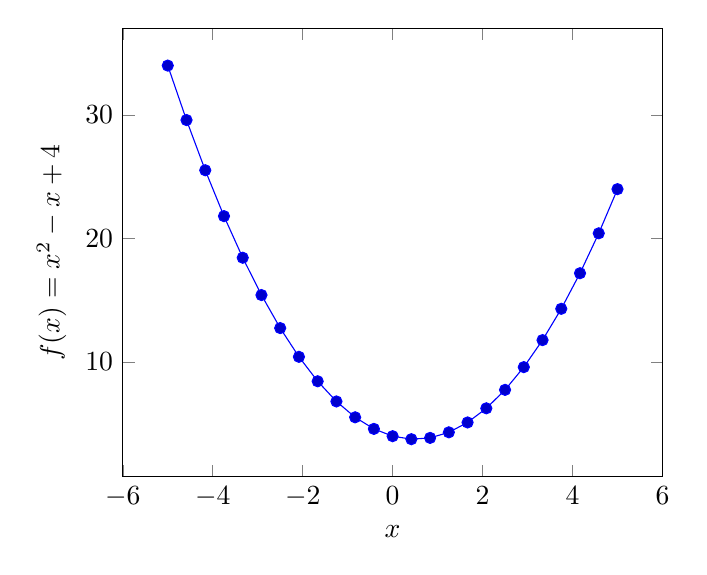
\begin{tikzpicture}
                \begin{axis}[
                    xlabel=$x$,
                    ylabel={$f(x) = x^2 - x +4$}
                ]
                % use TeX as calculator:
                \addplot {x^2 - x +4};
                \end{axis}
            \end{tikzpicture}
        }
        \subfloat[复杂的图像]{
            \begin{tikzpicture}
                \begin{axis}[scatter/classes={
                    a={mark=square*,blue},%
                    b={mark=triangle*,red},%
                    c={mark=o,draw=black}}]
                
                    % \addplot[] is better than \addplot+[] here:
                    % it avoids scalings of the cycle list
                    \addplot[scatter,only marks,
                        scatter src=explicit symbolic]
                        coordinates {
                            (0.1,0.15)  [a]
                            (0.45,0.27) [c]
                            (0.02,0.17) [a]
                            (0.06,0.1)  [a]
                            (0.9,0.5)   [b]
                            (0.5,0.3)   [c]
                            (0.85,0.52) [b]
                            (0.12,0.05) [a]
                            (0.73,0.45) [b]
                            (0.53,0.25) [c]
                            (0.76,0.5)  [b]
                            (0.55,0.32) [c]
                        };
                \end{axis}
            \end{tikzpicture}
        }
        \caption{pgfplots图像示例}
        \label{fig:pgfplots1}
    \end{figure}
    \section{贡献}
    本模板是本人按照学校提供的word模板修改而成,希望大家能在学习latex中进步,支持一下作者。

    %% 参考文献使用
    %设置参考文献风格,参照使用 https://github.com/Haixing-Hu/GBT7714-2005-BibTeX-Style
    % 一种是按照顺序的,一种是按照作者年月的
    \bibliographystyle{gbt7714-2005-author-year}
    \nocite{*}
    \bibliography{refers}
\end{document}

